% -*- mode: latex-mode -*-

% http://ctan.org/pkg/media9
\usepackage{media9}

\usepackage[utf8]{inputenc} % hyperref broken with utf8x
\usepackage[C40,T1]{fontenc}

\usepackage{lmodern}
\usepackage{graphicx}
\usepackage{array}
\usepackage{multirow}
\usepackage{overpic}
\usepackage{amsmath}

\usepackage{algorithmic, algorithm}

\usepackage{tikz}
\usetikzlibrary{calc,trees,positioning,arrows,chains,shapes.geometric,%
    decorations.pathreplacing,decorations.pathmorphing,shapes,%
    matrix,shapes.symbols}

\tikzset{
>=stealth',
  punktchain/.style={
    rectangle,
    rounded corners,
    % fill=black!10,
    draw=black, very thick,
    text width=10em,
    minimum height=3em,
    text centered,
    on chain},
  line/.style={draw, thick, <-},
  element/.style={
    tape,
    top color=white,
    bottom color=blue!50!black!60!,
    minimum width=8em,
    draw=blue!40!black!90, very thick,
    text width=10em,
    minimum height=3.5em,
    text centered,
    on chain},
  every join/.style={->, thick,shorten >=1pt},
  decoration={brace},
  tuborg/.style={decorate},
  tubnode/.style={midway, right=2pt},
}

% Remap the unicode indivisible space into a LateX tilde.
\DeclareUnicodeCharacter{00A0}{~}

% Customizme Beamer.
\usetheme{jrl}

% Set title, author, date.
\title[Motion Retargeting]{Optimization-based Motion Retargeting %
  Integrating Spatial and Dynamic Constraints}
\author[\emph{T.\ Moulard}, E.\ Yoshida, S.\ Nakaoka]{%
  Thomas Moulard, Eiichi Yoshida %
  \texorpdfstring{\\}{} and Shin'ichiro Nakaoka}

\institute{CNRS-AIST JRL UMI3218/CRT}

\date{Friday 25 October 2013}

% Setup pdf meta-data.
\hypersetup{
  pdfauthor = {Thomas Moulard},
  pdftitle = {Optimization-based Motion Retargeting Integrating Spatial and %
    Dynamic Constraints},
  pdfsubject = {Optimization-based Motion Retargeting Integrating Spatial and %
    Dynamic Constraints},
  pdfkeywords = {numerical optimization, humanoid robotics},
  pdfcreator = {Thomas Moulard},
  pdfproducer = {Thomas Moulard}
}

\begin{document}

\begin{frame}[plain]
  \titlepage
  \note[item]{Introduction, mention JSPS}
\end{frame}

\begin{frame}
  \tableofcontents
  \note[item]{I will start by explaining what is retargeting and why
  this is an important theme for us}
  \note[item]{then detail the issues we face}
  \note[item]{and show the results we obtained}
\end{frame}

\section{Problem Statement}
\begin{frame}
   \vfill
   \begin{center}
     \Large I. Problem Statement
   \end{center}
   \vfill
   \note[item]{First what is our motivation?}
\end{frame}

\begin{frame}
  \frametitle{Goal}

  \begin{columns}
    \column{.25\paperwidth}
    \includegraphics[width=.95\linewidth]{%
      assets/smartsuit.jpg}
    \par
    \includegraphics[width=.95\linewidth]{%
      assets/Honda-WAD.jpg}
    \column{.70\paperwidth}
    \begin{itemize}
    \item Smart Suits, Walking Assistive Device development is
      increasing.
    \item Humanoid Robots may help us validate their efficiency\ldots
    \item \ldots given that we can reproduce \textbf{human-like}
      motion.
    \end{itemize}
  \end{columns}

  \note[item]{Elderly people are an increasingly worrying issue.}
  \note[item]{Describe assistive devices / smart suits.}
\end{frame}

\begin{frame}
  \frametitle{\ldots on a Humanoid Robot}
  \begin{center}
    \includegraphics[width=.8\paperwidth]{%
      assets/hrp4c.jpg}
    \par
    HRP4C Humanoid Robot (1.58m, 45kg)
  \end{center}

  \note[item]{Describe HRP4-C goal}
\end{frame}



\begin{frame}
  \frametitle{Issues (I)}

  \begin{columns}
    \column{.45\paperwidth}
    \begin{center}
%    \includemedia[%
%      addresource=assets/HRP-4C_Human_like_walking.mp4,
%      width=.4\paperwidth,
%      flashvars={
%        flv=assets/HRP-4C_Human_like_walking.mp4
%        &autoPlay=true
%      },
%      activate=pageopen
%    ]{\includegraphics[%
%        width=.4\paperwidth,keepaspectratio]{%
%        assets/HRP-4C_Human_like_walking.jpg}}{player_flv_maxi.swf}%
%    \par
    \includegraphics[%
        width=.4\paperwidth,keepaspectratio]{%
        assets/motion-capture.jpg}
    \end{center}
    \column{.55\paperwidth}

    Testing on robot is\ldots
    \par
    \begin{description}
    \item[More Repeatable]~\\ no fatigue, etc.
    \item[Less Invasive]~\\ instrumentation is easier
    \item[Easier to Setup]~\\ cheaper and no ethical issues
    \end{description}
  \end{columns}

\end{frame}

\begin{frame}
  \begin{center}
    \includemedia[%
      addresource=assets/1810_smartsuit_2kg_trial01.mp4,
      width=.4\paperwidth,
      flashvars={
        flv=assets/1810_smartsuit_2kg_trial01.mp4
        &autoPlay=true
      },
      activate=pageopen
    ]{\includegraphics[%
        width=.4\paperwidth,keepaspectratio]{%
        assets/1810_smartsuit_2kg_trial01.jpg}}{player_flv_maxi.swf}%
    \includemedia[%
      addresource=assets/1746_smartsuit_2kg_trial01.mp4,
      width=.4\paperwidth,
      flashvars={
        flv=assets/1746_smartsuit_2kg_trial01.mp4
        &autoPlay=true
      },
      activate=pageopen
    ]{\includegraphics[%
        width=.4\paperwidth,keepaspectratio]{%
        assets/1746_smartsuit_2kg_trial01.jpg}}{player_flv_maxi.swf}%

    \footnotesize
    ~\includegraphics[height=.25cm]{assets/idea.pdf}~%
    Motion-Based-Design of Elastic Material for Passive Assistive Device
    Using Musculoskeletal Model
    (\mbox{Y.\ Imamura}, et al.),\\ Journal of Robotics and Mechatronics%
  \end{center}
\end{frame}

\begin{frame}
  \frametitle{Smartsuit Efficiency Evaluation}
  \begin{center}
    \begin{overpic}[width=.95\linewidth]{assets/exp-torque-smartsuit-chest.eps}
      \put(47,20){\usebeamercolor{alerted text}\rule{1pt}{30pt}}
      \put(67,20){\usebeamercolor{alerted text}\rule{1pt}{30pt}}
      \put(47,20){\usebeamercolor{alerted text}\linethickness{1pt}\line(1,0){20}}
    \end{overpic}
  \end{center}
\end{frame}


\begin{frame}
  \frametitle{Issues (II)}

  \begin{columns}
    \column{.35\paperwidth}
    \begin{center}
      \includegraphics[width=.34\paperwidth]{%
        assets/hrp4c-smartsuit2.jpg}
    \end{center}
    \column{.6\paperwidth}
    \begin{itemize}
    \item On a bending motion, torque reading is different on a
      bending motion with 2kg attached to robot wrists.
    \item Bending motion has been acquired through a motion capture
      system.
    \item Currently, manual motion tuning is required.
    \item How to automate this?
    \end{itemize}
    \par
    \footnotesize ~\includegraphics[height=.25cm]{assets/idea.pdf}~%
    Humanoid Robot as an Evaluator of Assistive Devices
    (K.\ Miura et al.), ICRA 2012
  \end{columns}
\end{frame}


\begin{frame}
  \frametitle{Adopted Strategy}

  \textbf{Motion Retargeting}

  \bigskip

  \begin{itemize}
  \item Use Motion Capture data from human actor.
  \item Reshape the motion so that it becomes reproducible by the robot.
    \begin{itemize}
    \item Different geometric structure, reduced number of degrees
      of freedom.
    \item Mass distributed differently, limited actuators
      capabilities (torque, velocity).
    \end{itemize}
  \end{itemize}

  \bigskip

  \footnotesize
  ~\includegraphics[height=.25cm]{assets/idea.pdf}~%
  Interaction Mesh Based Motion Adaptation for Biped Humanoid Robots
  (Shinichiro Nakaoka, Taku Komura), IEEE Humanoids 2012
\end{frame}


\section{Proposed Resolution Scheme}
\begin{frame}
   \vfill
   \begin{center}
     \Large II. Proposed Resolution Scheme
   \end{center}
   \vfill
\end{frame}

\begin{frame}
  \frametitle{Previous Work}

    \begin{columns}
    \column{.5\paperwidth}

    Formulate an optimization problem where constraints are
    ensuring feasibility while minimizing the changes.

    \begin{itemize}
    \item Previous work are mainly aiming image synthesis, not
      robotics.
    \item How to quantify changes in motion?
    \end{itemize}

    \column{.45\paperwidth}
    \includegraphics[width=.44\paperwidth]{%
      figure/InteractionMeshImage.png}
    \par
    \small
    \mbox{Interaction Mesh} can be used to quantify motion change.
  \end{columns}
\end{frame}

\begin{frame}
  \frametitle{Our Approach (I)}

  A non-linear optimization problem is solved.

  \begin{description}
  \item[Cost] Laplacian Deformation Energy
  \item[Constraints] ~\\
    \begin{itemize}
    \item Bone length
    \item Joint position, Velocity, \emph{Torque}
    \item \emph{Robot stability} (ZMP)
    \end{itemize}
  \end{description}
\end{frame}

\begin{frame}
  \frametitle{Our Approach (II)}

  \begin{center}
    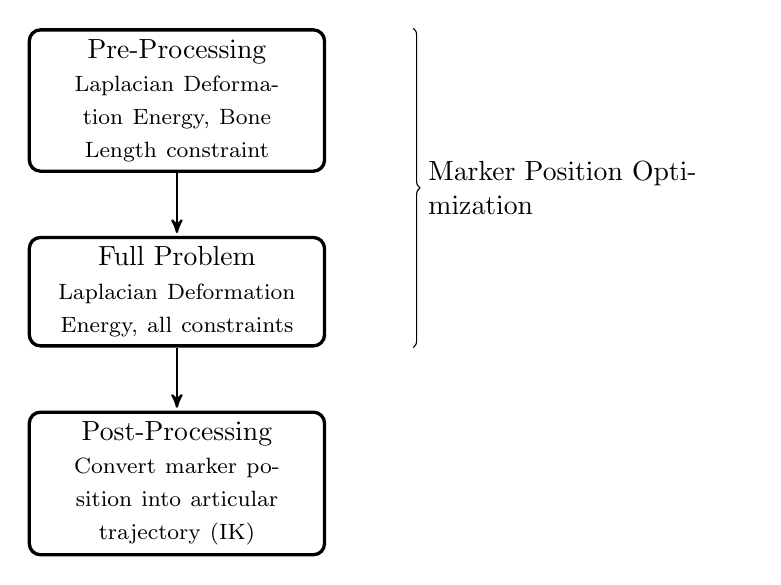
\begin{tikzpicture}
      [node distance=.8cm,
        start chain=going below,]
      \node[punktchain, join] (pre) {%
        \alert{Pre-Processing}\\
        \footnotesize
        Laplacian Deformation Energy, Bone Length constraint
      };
      \node[punktchain, join] (full) {%
        \alert{Full Problem}\\
        \footnotesize
        Laplacian Deformation Energy, all constraints
      };
      \node[punktchain, join] (post) {%
        \alert{Post-Processing}\\
        \footnotesize
        Convert marker position into articular trajectory (IK)};

      \draw[tuborg, decoration={brace}] let \p1=(pre.north), \p2=(full.south) in
      ($(3, \y1)$) -- ($(3, \y2)$) node[tubnode,text width=4cm] {%
        Marker Position Optimization
      };
    \end{tikzpicture}
  \end{center}
\end{frame}


\begin{frame}
  \frametitle{Constraints}

  \alert{Joint Position}\\
  \ldots in actuators limits.

  \bigskip

  \alert{Joint Velocity}\\
  \ldots in actuators limits.

  \bigskip

  \alert{Joint Torque}~\\
  \ldots in actuators limits.\\
  Computed from links position, velocity and acceleration (Inverse
  Dynamics algorithm).

  \bigskip

  \alert{ZMP}\\
  \ldots must be in the polygon support to ensure dynamic stability of the
  motion. Computed from links position, velocity and acceleration.
\end{frame}

\section{Simulation and Conclusion}
\begin{frame}
   \vfill
   \begin{center}
     \Large III. Simulation and Conclusion
   \end{center}
   \vfill
\end{frame}

\begin{frame}
  \frametitle{Marker Position Optimization}

  \begin{columns}
    \column{.45\paperwidth}
    \begin{center}
      \includegraphics[width=.22\paperwidth]{%
        figure/before.png}
      \includegraphics[width=.22\paperwidth]{%
        figure/after.png}
      \par
      \small
      Before (left) and After (right) optimization.
    \end{center}
    \column{.45\paperwidth}

    Trying to optimize the motion capture markers position directly.

    \begin{itemize}
      \item Torque and ZMP constraints are hard to express.
      \item The problem is difficult (and slow) to solve.
    \end{itemize}
  \end{columns}
\end{frame}

\begin{frame}
  \frametitle{Joint Value Optimization (new) (I)}

  \begin{columns}
    \column{.45\paperwidth}
    \begin{center}
      \includegraphics[width=.44\paperwidth]{%
        figure/retargeting-preprocessing.jpg}
      \par
%      \includegraphics[width=.22\paperwidth]{%
%        figure/retargeting-result1.jpg}
%      \par
      \small
      Before (pink) and After (grey) pre-processing.
    \end{center}

    \column{.45\paperwidth}
    Optimizing the joint values.

    \begin{itemize}
    \item Solve a linear optimization problem which will adapt
      the motion to the robot morphology.
    \item The optimization result is used at the starting point
      of the non-linear problem.
    \end{itemize}
  \end{columns}
\end{frame}

\begin{frame}
  \frametitle{Joint Value Optimization (new) (II)}

  \begin{center}
    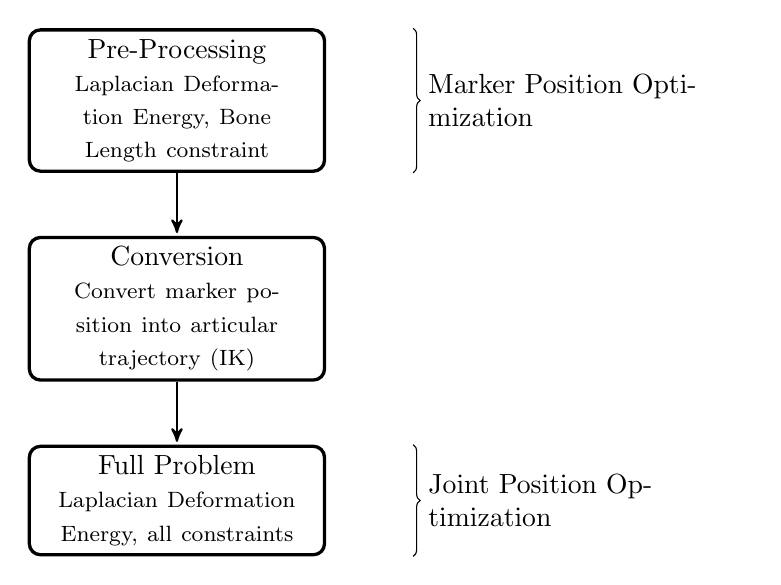
\begin{tikzpicture}
      [node distance=.8cm,
        start chain=going below,]
      \node[punktchain, join] (pre) {%
        \alert{Pre-Processing}\\
        \footnotesize
        Laplacian Deformation Energy, Bone Length constraint
      };
      \node[punktchain, join] (post) {%
        \alert{Conversion}\\
        \footnotesize
        Convert marker position into articular trajectory (IK)};
      \node[punktchain, join] (full) {%
        \alert{Full Problem}\\
        \footnotesize
        Laplacian Deformation Energy, all constraints
      };

      \draw[tuborg, decoration={brace}] let \p1=(pre.north), \p2=(pre.south) in
      ($(3, \y1)$) -- ($(3, \y2)$) node[tubnode,text width=4cm] {%
        Marker Position Optimization
      };
      \draw[tuborg, decoration={brace}] let \p1=(full.north), \p2=(full.south) in
      ($(3, \y1)$) -- ($(3, \y2)$) node[tubnode,text width=3cm] {%
        Joint Position Optimization
      };
    \end{tikzpicture}
  \end{center}
\end{frame}



\begin{frame}
  \frametitle{Results (I)}

  \begin{itemize}
  \item The new approach is still work in progress.
  \item Preliminary results are promising.
  \item Probable that near real-time optimization can be achieved.
  \end{itemize}

\end{frame}

\begin{frame}
  \frametitle{Results (II)}

    \begin{columns}
    \column{.49\paperwidth}
    \begin{center}
      \includemedia[%
        addresource=assets/hrp4c-retargeting.mp4,
        width=.99\linewidth,
        flashvars={
          flv=assets/hrp4c-retargeting.mp4
          &autoPlay=true
        },
        activate=pageopen
      ]{\includegraphics[%
          width=.9\linewidth,keepaspectratio]{%
          assets/hrp4c-retargeting.jpg}}{player_flv_maxi.swf}%
    \end{center}
    \column{.49\paperwidth}
    \begin{center}
      \begin{overpic}[width=.99\linewidth]{assets/zmp.pdf}
        \put(32,15){\usebeamercolor{alerted text}\linethickness{1pt}\line(0,1){30}}

        \put(74,15){\usebeamercolor{alerted text}\linethickness{1pt}\line(0,1){30}}

        \put(32,45){\usebeamercolor{alerted text}\linethickness{1pt}\line(1,0){42}}
        \put(32,15){\usebeamercolor{alerted text}\linethickness{1pt}\line(1,0){42}}
      \end{overpic}
    \end{center}
    \end{columns}

    \bigskip

    \begin{center}
      Optimizing a fast arm motion\\
      inducing kinematic momentum (display: geometric simulation only).
    \end{center}
\end{frame}


\begin{frame}
  \frametitle{Conclusion}

  \begin{itemize}
  \item Proposed scheme allow to automatically process a motion to
    adapt it to any humanoid robot without needing any human
    intervention.
  \item This may be used to reproduce human-like motion on humanoid
    robots which is useful, for instance, to study walking assistive
    devices.
  \item Marker space optimization is computationally intense: a new
    approach with joint space optimization is in progress.
  \end{itemize}
\end{frame}

\maxFrameImage{assets/hrp2-thx.jpg}

\begin{frame}[noframenumbering]
  \frametitle{Walking Assistive Device}

  \begin{columns}
    \column{.45\paperwidth}
    \begin{center}
      \includegraphics[width=.35\paperwidth]{%
        assets/Honda-WAD.jpg}
      \par
      Honda Walk Assist
    \end{center}
    \column{.45\paperwidth}
    \begin{center}
      \includegraphics[width=.33\paperwidth]{%
        assets/cyberdine.jpg}
      \par
      Cyberdine HAL
    \end{center}
  \end{columns}
\end{frame}

\begin{frame}
  \frametitle{Optimization Problem}

  \begin{multline}
    \min_{\mathbf{x} \in \mathbb{R}^n} \text{LDE}(\Gamma(\mathbf{x})) \text{ s.t. }\\
    \begin{cases}
      \Gamma_{\mathbf{x}}(t))
      \in [\mathbf{q}_{\text{lower}}, \mathbf{q}_{\text{upper}}]\\
      \dot{\Gamma}_{\mathbf{x}}(t))
      \in [\dot{\mathbf{q}}_{\text{lower}}, \dot{\mathbf{q}}_{\text{upper}}]\\
      \tau(\ddot{\Gamma}_{\mathbf{x}}(t)),
      \dot{\Gamma}_{\mathbf{x}}(t)),\Gamma_{\mathbf{x}}(t)))
      \in [\mathbf{\tau}_{\text{lower}}, \mathbf{\tau}_{\text{lower}}]\\
      \text{ZMP}(\ddot{\Gamma}_{\mathbf{x}}(t)),
      \dot{\Gamma}_{\mathbf{x}}(t)),\Gamma_{\mathbf{x}}(t)))
      \in \mathcal{P}_s\\
    \end{cases}
  \end{multline}
\end{frame}


\begin{frame}
  \frametitle{Cost Function}

  \alert{Laplacian Deformation Energy} quantify the interaction mesh
  deformation.

  \begin{equation}
    E_L(\mathbf{m}) = \sum_i \frac{1}{2} \| \mathbf{\delta}_i - L(\mathbf{m}_i) \|^2
  \end{equation}

  \begin{equation}
    L(\mathbf{m}_i) = \mathbf{m}_i - \sum_j w_{(i,j)} \mathbf{m}_j
  \end{equation}

  $m_i$ the $i$-th marker Euclidian position.\\
  $\mathbf{\delta}_i$ the original Laplacian Coordinate of the $i$-th marker.\\
  $w_{(i,j)}$ the weight of the $(i,j)$ link in the interaction mesh.
\end{frame}


\end{document}
